%
\documentclass[%
 reprint,
 amsmath,amssymb,
 aps,
]{revtex4-1}

\usepackage{graphicx}% Include figure files
\usepackage{dcolumn}% Align table columns on decimal point
\usepackage{bm}% bold math


\begin{document}


\title{Comparativa Metodologia Kimball vs Metodología Inmon}
\author{Robles Flores, Anthony Richard	               (2016056192)}
\author{Estrella Palacios, Katherine Lizbeth			(2015050948)}
\author{Sosa Bedoya, Sharon Fiorela					(2016054460)}
\author{Torres Beltran , Johanna Andrea				(2020067849)}

		
\affiliation{%
 Universidad Privada de Tacna \textbackslash Facultad de Ingenieria \textbackslash Escuela Profesional de Ingenieria de Sistemas
}%

\begin{abstract}
\begin{center}
\textbf{Resumen}
\end{center}
Los almacenes de datos (data warehouses en inglés) toman cada día mayor importancia, a medida que las organizaciones pasan de esquemas de sólo recolección de datos a esquemas de análisis de los mismos. En este breve artículo se  tratará de brindar una explicación general de algunas metodologías, en este caso serán la metodología Kimball y la metodología Inmon.
\\

\begin{center}
\textbf{Abstract}
\end{center}
Data warehouses (data warehouses in English) are becoming increasingly important, as organizations move from data-only schemes to data analysis schemes. In this short article we will try to provide a general explanation of some methodologies, in this case they will be the Kimball methodology and the Inmon methodology.
\\
\end{abstract}



\maketitle

%\tableofcontents

\section {Introducción}\label{sec:1}

Actualmente las organizaciones utilizan la información y el conocimiento para apoyar la toma de sus decisiones estratégicas, y de este modo lograr sus metas y mejorar sus procesos.
Uno de los desafíos que enfrentan hoy las organizaciones, es el aumento de datos, lo que ha generado dos grandes problemas; el primero, identificar los datos relevantes para dar seguimiento a su estrategia organizacional, y lograr que se cumplan los planes con las metas establecidas.
 Y el segundo problema, la capacidad para administrar esta gran cantidad de datos.
Un almacén de datos  según Inmon, es una colección de datos orientada a un determinado ámbito (empresa, organización, etc.), integrado, no volatil y variable en el tiempo, que ayuda a la toma de decisiones en la entidad en la que se utiliza. 
Se trata, sobre todo, de un historial completo de la organización, mas alla de la informacion transaccional y operacional, almacenado en una base de datos diseñada para favorecer el análisis y la divulgación eficiente de datos (especialmente con herramientas OLAP, de procesamiento analítico en línea). Por otra parte Kimball la define como una copia de los datos transaccionales estructurados específicamente para consultas y análisis. 
En este breve artículo intentaremos brindar una explicación general de dos de las metodologías más usadas, la metodología de Kimball y metodología Inmon. \cite{estrella1}
%-----------------------------------------------------------------
\section{Objetivos}\label{sec:2}
\subsection{General:}
Dar una visión clara de BI, desde las perspectivas de los autores que sentaron las bases que son Ralph Kimball y Bill Inmon, para la mejora de las estrategias del negocio al que se desee implementar las herramientas de BI.
\subsection{Específicos:}
 Describir las metodologías propuestas por los principales autores de BI desde las perspectivas de sus creadores Ralph Kimball y Bill Inmon.


%-----------------------------------------------------------------
\section {Marco Teórico}

\subsection{METODOLOGIA SEGUN INMON}	
Un almacén de datos (data warehouse, DW) según Inmon es una colección de datos orientada a un determinado ámbito (empresa, organización, etc.), integrado, no volátil y variable en el tiempo, que ayuda a la toma de decisiones en la entidad en la que se utiliza. Se trata, sobre todo, de un historial completo de la organización, más allá de la información transaccional y operacional, almacenado en una base de datos diseñada para favorecer el análisis y la divulgación eficiente de datos (especialmente con herramientas OLAP, de procesamiento analítico en línea). \cite{estrella2}

Consta de las siguientes características:
\begin{itemize}
		\item \textbf{Orientado a temas:} Los datos en la base de datos están organizados de manera que todos los elementos de datos relativos al mismo evento u objeto del mundo real queden unidos entre sí.
		\item \textbf{Integrado:} La base de datos contiene los datos de todos los sistemas operacionales de la organización, y dichos datos deben ser consistentes. 
		\item \textbf{No volátil:} La información no se modifica ni se elimina, una vez almacenado un dato, éste se convierte en información de sólo lectura, y se 	mantiene para futuras consultas.
		\item \textbf{Variante en el tiempo:}Los cambios producidos en los datos a lo largo del tiempo quedan registrados para que los informes que se puedan generar reflejen esas variaciones.

\end{itemize}


El enfoque Inmon tambien se referencia normalmente como Top-down. Los datos son extraidos de los sistemas operacionales por los procesos ETL y cargados en las areas de stage, donde son validados y consolidados en el DW corporativo, donde ademas existen los llamados metadatos que documentan de una forma clara y precisa el contenido del DW. Una vez realizado este proceso, los procesos de refresco de los Data Mart departamentales obtienen la información de el, y con las consiguientes transformaciones, organizan los datos en las estructuras particulares requeridas por cada uno de ellos, refrescando su contenido.


%-------------------------------------------------

\subsection{IMPLEMENTACIONES DE  INMON}
\begin{itemize}
	\item Descomposición funcional
	\item Diagrama de contexto
	\item Diagrama de flujo de datos
	\item Diagrama de transición de estados
	\item Pseudocódigo
\end{itemize}

	c. Modelo de datos. Se trabaja con 2 tipos de modelos:
		\begin{itemize}
			\item El Modelo de datos nos muestra los datos primitivos, tomando en cuenta el elemento tiempo, se plasman los cálculos que se realicen y finalmente se muestran sus relaciones.
		\end{itemize}

El Modelo de Datos del Data Warehouse. Los modelos anteriores nos deberán entregar la definición de los sujetos a los que estará orientado el Data Warehouse. Debe venir en 3 perspectivas y son explicadas en la siguiente tabla:


	d. Una vez que se tiene conocimiento de este modelo se deben tomar ciertas decisiones sobre el diseño del Data Warehouse. Entre estas decisiones tenemos las siguientes:
		\begin{itemize}
			\item Normalización, debemos decidir el grado al que nuestro Data Warehouse
			\item Granularidad
			\item Particiones
			\item  Minería de Datos
		\end{itemize}

	e. Al haber tomado estas decisiones, se debe generar un documento que contenga estas decisiones que hemos tomado para la definición del Data Warehouse. Este documento debe contener un concepto de Data Warehouse, una descripción de los sistemas que lo alimentan, como se debe usar el Data Warehouse, como obtener ayuda, responsables, plan de migración, mapeo de datos entre los datos operacionales y el data Warehouse, etc.

	f. Metadata. Contiene información sobre nuestro Data Warehouse. En pocas palabras es un diccionario de datos. Es pieza clave para el mejor aprovechamiento del Data Warehouse. Facilita las tareas de análisis ya que funciona como un índice del contenido del Data Warehouse.

2. Integración de datos. Implica el implementar procesos ETL que nos permitan extraer la información de los ambientes transacciones para cargarlo dentro del Data Warehouse. Esto puede implicar un cambio en la tecnología, selección de los datos que residirán en el Data Warehouse, cambios de llaves en los objetos, formato de los datos, sumarizaciones, estandarización de nomenclaturas.

3. Pruebas. Se hacen pruebas al respecto de la implementación del Data Warehouse. Se realizan los ajustes necesarios para poder obtener los resultados esperados en nuestro Data Warehouse.

4. Programación. Se hacen las programaciones necesarias para que se ejecuten ciertos procesos, para que exista la posibilidad de paralelismo, se administra la Meta Data, índices, particiones, monitoreo, etc.

5. Diseño DSS. Se trabaja sobre un esquema multidimensional para poder generar la información que realmente soporte la toma de decisiones.

6. Análisis. El tomador de decisiones analiza la información obtenida a partir del DSS.

7. Requerimientos. A partir del análisis de los datos obtenidos el tomador de decisiones llegue al entendimiento de los requerimientos que tiene su negocio para mejorar. A grandes rasgos esta es la metodología que Bill Inmon propone y que forma parte del marco de referencia de este trabajo de investigación.

%-------------------------------------------------
\subsection{ARQUITECTURA SEGUN INMON}
\begin{figure}[htb]
				\begin{center}
					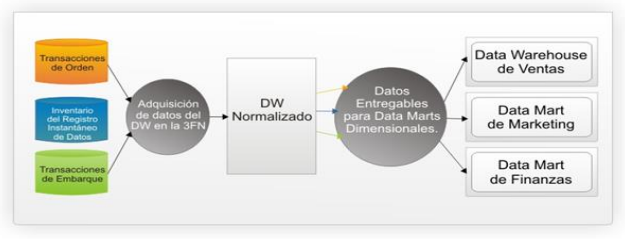
\includegraphics[width=9cm]{./IMAGENES/imgleydi2}
				\end{center}
			\end{figure}

La arquitectura que plantea Bill Inmon consta de las siguientes partes: \cite{robles1}

\begin{itemize}
		\item Fuente de la Información: Inicia el proceso de creación de un DW, conociendo la información que se necesita de todas las herramientas de las que se tengan acceso, ir a las necesidades de información que se necesitan con la finalidad de un resultado para crear un DW.

		\item Data Warehouse: La necesidad de normalizar toda la información extraída para ser almacenada en un DW, los cuales serán procesados y consultados por un DM.
		\item Data Marts: Se crean un subconjunto de los datos de un DW con el objetivo de responder a un determinado análisis o necesidad de una población, de un departamento en específico.
		\item Explotación de los datos: Se refiere a la manera de presentación de la información para ser consultada y analizada por las áreas. En cuanto a la arquitectura interna de un DW, Bill Inmon considera las siguientes características:

			\begin{itemize}
				\item Normalización: el DW debe ser basado y diseñado, conforme al diseño de las bases de datos transaccionales con las que se esté interactuando.
				\item Tercera Forma normal: la prioridad es que el modelo de datos esté construido en TFN con lo cual se tenga mayor relación entre los objetos de la base de datos.
			\end{itemize}

\end{itemize}

\subsection{La estructura del DataWarehouse}	
En cuanto a la estructura interna del DataWarehouse, para Inmon la prioridad es que el modelo de datos esté construido en tercera forma normal. Por dar una breve explicación de lo que esto significa, el proceso de normalización consiste en aplicar una serie de reglas o normas a la hora de establecer las relaciones entre los diferentes objetos dentro de la base de datos. Con este proceso de normalización se consiguen muchos beneficios, como evitar la redundancia de los datos, mantener su integridad referencial, facilitar el mantenimiento de las tablas y disminuir el tamaño de la base de datos. Sin embargo, a diferencia de los DataWarehouse desnormalizados, las consultas exigen el empleo de queries mucho más complejas, lo que dificulta el análisis directo de la información y el uso de las herramientas de reporting. De ahí, la necesidad de construir los DataMarts que, como ya comenté, están basados en modelos dimensionales de estrella o copo de nieve, diseños fácilmente explotables por estas herramientas de análisis de datos.\cite{aquino}

			\begin{figure}[htb]
				\begin{center}
					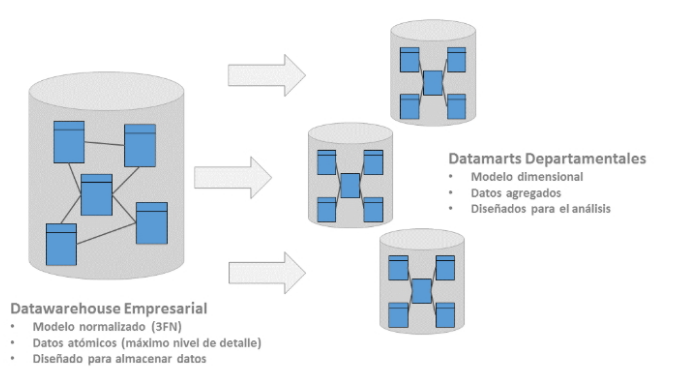
\includegraphics[width=9cm]{./IMAGENES/imgleydi3}
				\end{center}
			\end{figure}
%-------------------------------------------------
\subsection{METODOLOGIA SEGUN KIMBALL}	
xxxxxxxxxxxxxxxxxxxxxxxxxxxxxxxxxxxxxx 

%-------------------------------------------------
\subsection{IMPLEMENTACIONES DE KIMBALL}
xxxxxxxxxxxxxxxxxxxxxxxxxxxxxxxxxxxxxx 

%-------------------------------------------------
\subsection{ARQUITECTURA SEGUN KIMBALL}

xxxxxxxxxxxxxxxxxxxxxxxxxxxxxxxxxxxxxx 

%-------------------------------------------------

\subsection{COMPARACION DE METODOLOGIAS}	
xxxxxxxxxxxxxxxxxxxxxxxxxxxxxxxxxxxxxx

%-----------------------------------------------------------------
\section{Análisis}

\begin{itemize}
\item xxxxxxxxxxxxxxxxxxxxxxxxxxxxxxxxxxxxxx 
\item xxxxxxxxxxxxxxxxxxxxxxxxxxxxxxxxxxxxxx 
\end{itemize}
%-----------------------------------------------------------------
\section{Conclusiones}

\begin{itemize}
\item xxxxxxxxxxxxxxxxxxxxxxxxxxxxxxxxxxxxxx 
\item xxxxxxxxxxxxxxxxxxxxxxxxxxxxxxxxxxxxxx 

\end{itemize}


% Bibliografia.
%-----------------------------------------------------------------

\bibliographystyle{apalike}

\bibliography{Bibliografia}

\end{document}
